\documentclass[11pt,]{article}
\usepackage{lmodern}
\usepackage{amssymb,amsmath}
\usepackage{ifxetex,ifluatex}
\usepackage{fixltx2e} % provides \textsubscript
\ifnum 0\ifxetex 1\fi\ifluatex 1\fi=0 % if pdftex
  \usepackage[T1]{fontenc}
  \usepackage[utf8]{inputenc}
\else % if luatex or xelatex
  \ifxetex
    \usepackage{mathspec}
  \else
    \usepackage{fontspec}
  \fi
  \defaultfontfeatures{Ligatures=TeX,Scale=MatchLowercase}
\fi
% use upquote if available, for straight quotes in verbatim environments
\IfFileExists{upquote.sty}{\usepackage{upquote}}{}
% use microtype if available
\IfFileExists{microtype.sty}{%
\usepackage{microtype}
\UseMicrotypeSet[protrusion]{basicmath} % disable protrusion for tt fonts
}{}
\usepackage[margin=1in]{geometry}
\usepackage{hyperref}
\hypersetup{unicode=true,
            pdftitle={Assignment 6, EDDA 2017},
            pdfauthor={Martin de la Riva(11403799) and Kieran O'Driscoll(11426438), Group 23},
            pdfborder={0 0 0},
            breaklinks=true}
\urlstyle{same}  % don't use monospace font for urls
\usepackage{color}
\usepackage{fancyvrb}
\newcommand{\VerbBar}{|}
\newcommand{\VERB}{\Verb[commandchars=\\\{\}]}
\DefineVerbatimEnvironment{Highlighting}{Verbatim}{commandchars=\\\{\}}
% Add ',fontsize=\small' for more characters per line
\usepackage{framed}
\definecolor{shadecolor}{RGB}{248,248,248}
\newenvironment{Shaded}{\begin{snugshade}}{\end{snugshade}}
\newcommand{\KeywordTok}[1]{\textcolor[rgb]{0.13,0.29,0.53}{\textbf{{#1}}}}
\newcommand{\DataTypeTok}[1]{\textcolor[rgb]{0.13,0.29,0.53}{{#1}}}
\newcommand{\DecValTok}[1]{\textcolor[rgb]{0.00,0.00,0.81}{{#1}}}
\newcommand{\BaseNTok}[1]{\textcolor[rgb]{0.00,0.00,0.81}{{#1}}}
\newcommand{\FloatTok}[1]{\textcolor[rgb]{0.00,0.00,0.81}{{#1}}}
\newcommand{\ConstantTok}[1]{\textcolor[rgb]{0.00,0.00,0.00}{{#1}}}
\newcommand{\CharTok}[1]{\textcolor[rgb]{0.31,0.60,0.02}{{#1}}}
\newcommand{\SpecialCharTok}[1]{\textcolor[rgb]{0.00,0.00,0.00}{{#1}}}
\newcommand{\StringTok}[1]{\textcolor[rgb]{0.31,0.60,0.02}{{#1}}}
\newcommand{\VerbatimStringTok}[1]{\textcolor[rgb]{0.31,0.60,0.02}{{#1}}}
\newcommand{\SpecialStringTok}[1]{\textcolor[rgb]{0.31,0.60,0.02}{{#1}}}
\newcommand{\ImportTok}[1]{{#1}}
\newcommand{\CommentTok}[1]{\textcolor[rgb]{0.56,0.35,0.01}{\textit{{#1}}}}
\newcommand{\DocumentationTok}[1]{\textcolor[rgb]{0.56,0.35,0.01}{\textbf{\textit{{#1}}}}}
\newcommand{\AnnotationTok}[1]{\textcolor[rgb]{0.56,0.35,0.01}{\textbf{\textit{{#1}}}}}
\newcommand{\CommentVarTok}[1]{\textcolor[rgb]{0.56,0.35,0.01}{\textbf{\textit{{#1}}}}}
\newcommand{\OtherTok}[1]{\textcolor[rgb]{0.56,0.35,0.01}{{#1}}}
\newcommand{\FunctionTok}[1]{\textcolor[rgb]{0.00,0.00,0.00}{{#1}}}
\newcommand{\VariableTok}[1]{\textcolor[rgb]{0.00,0.00,0.00}{{#1}}}
\newcommand{\ControlFlowTok}[1]{\textcolor[rgb]{0.13,0.29,0.53}{\textbf{{#1}}}}
\newcommand{\OperatorTok}[1]{\textcolor[rgb]{0.81,0.36,0.00}{\textbf{{#1}}}}
\newcommand{\BuiltInTok}[1]{{#1}}
\newcommand{\ExtensionTok}[1]{{#1}}
\newcommand{\PreprocessorTok}[1]{\textcolor[rgb]{0.56,0.35,0.01}{\textit{{#1}}}}
\newcommand{\AttributeTok}[1]{\textcolor[rgb]{0.77,0.63,0.00}{{#1}}}
\newcommand{\RegionMarkerTok}[1]{{#1}}
\newcommand{\InformationTok}[1]{\textcolor[rgb]{0.56,0.35,0.01}{\textbf{\textit{{#1}}}}}
\newcommand{\WarningTok}[1]{\textcolor[rgb]{0.56,0.35,0.01}{\textbf{\textit{{#1}}}}}
\newcommand{\AlertTok}[1]{\textcolor[rgb]{0.94,0.16,0.16}{{#1}}}
\newcommand{\ErrorTok}[1]{\textcolor[rgb]{0.64,0.00,0.00}{\textbf{{#1}}}}
\newcommand{\NormalTok}[1]{{#1}}
\usepackage{graphicx,grffile}
\makeatletter
\def\maxwidth{\ifdim\Gin@nat@width>\linewidth\linewidth\else\Gin@nat@width\fi}
\def\maxheight{\ifdim\Gin@nat@height>\textheight\textheight\else\Gin@nat@height\fi}
\makeatother
% Scale images if necessary, so that they will not overflow the page
% margins by default, and it is still possible to overwrite the defaults
% using explicit options in \includegraphics[width, height, ...]{}
\setkeys{Gin}{width=\maxwidth,height=\maxheight,keepaspectratio}
\IfFileExists{parskip.sty}{%
\usepackage{parskip}
}{% else
\setlength{\parindent}{0pt}
\setlength{\parskip}{6pt plus 2pt minus 1pt}
}
\setlength{\emergencystretch}{3em}  % prevent overfull lines
\providecommand{\tightlist}{%
  \setlength{\itemsep}{0pt}\setlength{\parskip}{0pt}}
\setcounter{secnumdepth}{0}
% Redefines (sub)paragraphs to behave more like sections
\ifx\paragraph\undefined\else
\let\oldparagraph\paragraph
\renewcommand{\paragraph}[1]{\oldparagraph{#1}\mbox{}}
\fi
\ifx\subparagraph\undefined\else
\let\oldsubparagraph\subparagraph
\renewcommand{\subparagraph}[1]{\oldsubparagraph{#1}\mbox{}}
\fi

%%% Use protect on footnotes to avoid problems with footnotes in titles
\let\rmarkdownfootnote\footnote%
\def\footnote{\protect\rmarkdownfootnote}

%%% Change title format to be more compact
\usepackage{titling}

% Create subtitle command for use in maketitle
\newcommand{\subtitle}[1]{
  \posttitle{
    \begin{center}\large#1\end{center}
    }
}

\setlength{\droptitle}{-2em}
  \title{Assignment 6, EDDA 2017}
  \pretitle{\vspace{\droptitle}\centering\huge}
  \posttitle{\par}
  \author{Martin de la Riva(11403799) and Kieran O'Driscoll(11426438), Group 23}
  \preauthor{\centering\large\emph}
  \postauthor{\par}
  \predate{\centering\large\emph}
  \postdate{\par}
  \date{18 May 2017}


\begin{document}
\maketitle

\section{Assignment 6}\label{assignment-6}

\subsection{Exercise 1}\label{exercise-1}

\begin{Shaded}
\begin{Highlighting}[]
\NormalTok{fruitflies=}\KeywordTok{read.table}\NormalTok{(}\StringTok{'fruitflies.txt'}\NormalTok{, }\DataTypeTok{header=}\OtherTok{TRUE}\NormalTok{)}
\NormalTok{fruitflies$loglongevity <-}\StringTok{ }\KeywordTok{log}\NormalTok{(fruitflies$longevity)}
\end{Highlighting}
\end{Shaded}

\subsubsection{2.}\label{section}

\begin{Shaded}
\begin{Highlighting}[]
\KeywordTok{plot}\NormalTok{(loglongevity~thorax, }\DataTypeTok{pch=}\KeywordTok{as.character}\NormalTok{(activity), }\DataTypeTok{col=}\KeywordTok{as.numeric}\NormalTok{(activity), }\DataTypeTok{data=}\NormalTok{fruitflies)}
\KeywordTok{abline}\NormalTok{(}\KeywordTok{lm}\NormalTok{(loglongevity~thorax, }\DataTypeTok{data=}\NormalTok{fruitflies), }\DataTypeTok{col=}\StringTok{"blue"}\NormalTok{)}
\end{Highlighting}
\end{Shaded}

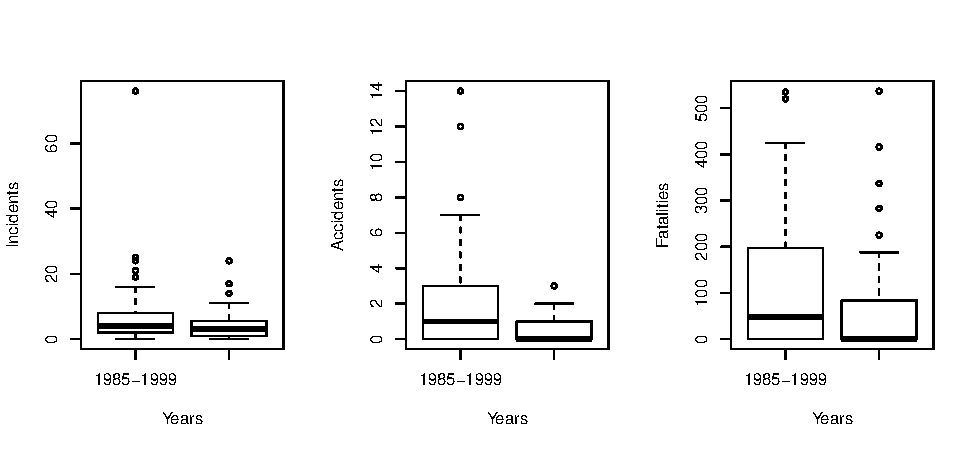
\includegraphics{assignment6_files/figure-latex/unnamed-chunk-2-1.pdf}

In the plot above, longevity seems to increase with torax.

\begin{Shaded}
\begin{Highlighting}[]
\CommentTok{# per activity:}
\KeywordTok{boxplot}\NormalTok{(fruitflies$loglongevity~fruitflies$activity)}
\end{Highlighting}
\end{Shaded}

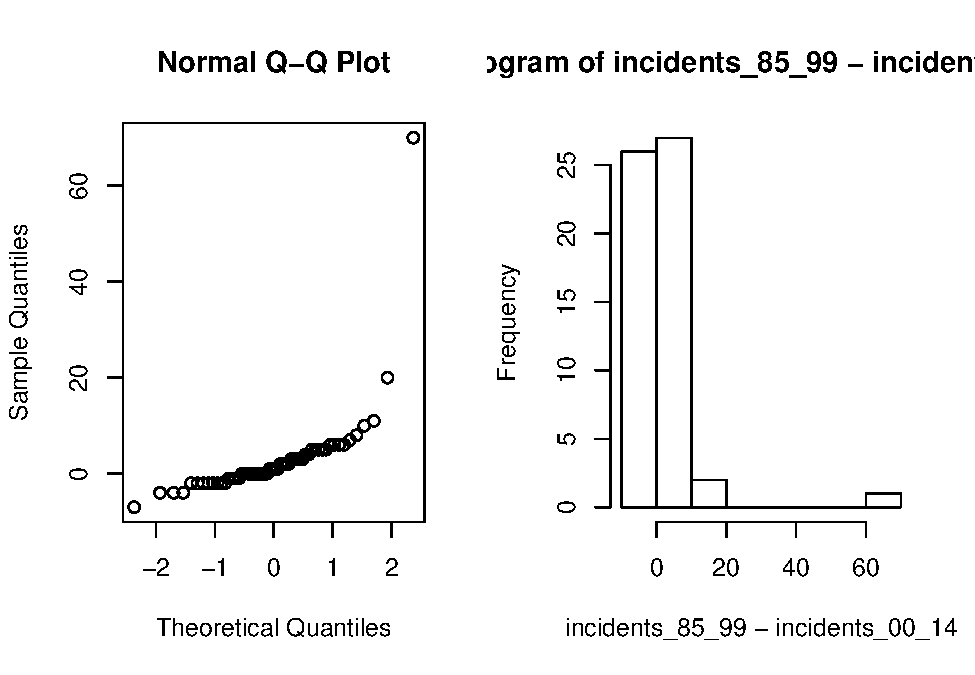
\includegraphics{assignment6_files/figure-latex/unnamed-chunk-3-1.pdf}

In these boxplots, it can be seen how high activity has a significantly
low longevity than low and isolated activity. Those two last activities
remain in similar longevity values.

\begin{Shaded}
\begin{Highlighting}[]
\CommentTok{# thorax per activity (is there a significant difference between them?)}
\KeywordTok{boxplot}\NormalTok{(fruitflies$thorax~fruitflies$activity)}
\end{Highlighting}
\end{Shaded}

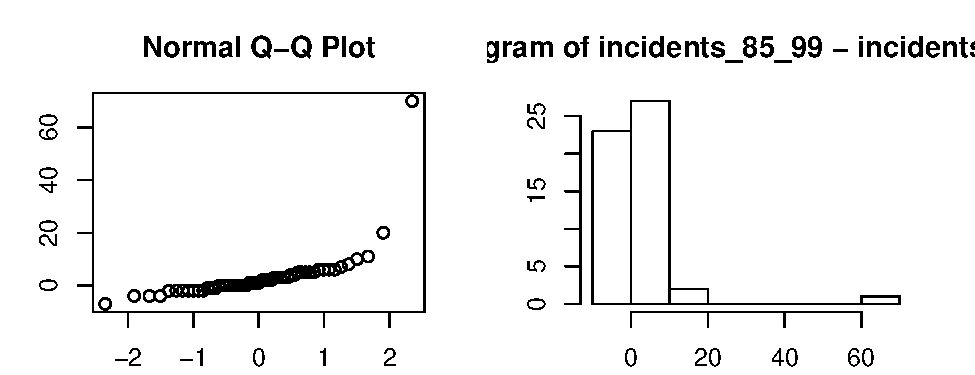
\includegraphics{assignment6_files/figure-latex/unnamed-chunk-4-1.pdf}

Lastly, we plot activity with respect to thorax, to see if thorax
lengths are equally distributed along the activity groups. This is
important, as if one group was full of bigger thorax fruitflies, this
could affect the result of the experiment. The activity groups are seen
to actually have similar thorax values.

\subsubsection{3.}\label{section-1}

\begin{Shaded}
\begin{Highlighting}[]
\NormalTok{flieslm =}\StringTok{ }\KeywordTok{lm}\NormalTok{(loglongevity~activity, }\DataTypeTok{data=}\NormalTok{fruitflies)}
\KeywordTok{anova}\NormalTok{(flieslm)}
\end{Highlighting}
\end{Shaded}

\begin{verbatim}
## Analysis of Variance Table
## 
## Response: loglongevity
##           Df Sum Sq Mean Sq F value    Pr(>F)    
## activity   2 3.6665  1.8333  19.421 1.798e-07 ***
## Residuals 72 6.7966  0.0944                      
## ---
## Signif. codes:  0 '***' 0.001 '**' 0.01 '*' 0.05 '.' 0.1 ' ' 1
\end{verbatim}

Sexual activity seems to significantly influence longevity, with a
p-value of 1.798e-07.

\subsubsection{4.}\label{section-2}

\begin{Shaded}
\begin{Highlighting}[]
\KeywordTok{confint}\NormalTok{(flieslm)}
\end{Highlighting}
\end{Shaded}

\begin{verbatim}
##                      2.5 %    97.5 %
## (Intercept)      3.4796296 3.7246190
## activityisolated 0.3439909 0.6904582
## activitylow      0.2244780 0.5709453
\end{verbatim}

The more sexual activity the less longetivity. In the Confidence
Intervals for the different activities, this can be seen: Confidence
Intervals for \(\mu_{high}\) activity: {[}3.4796296, 3.7246190{]}
Confidence Intervals for \(\mu_{isolated}\) - \(\mu_{high}\):
{[}0.3439909, 0.6904582{]} Confidence Intervals for \(\mu_{low}\) -
\(\mu_{high}\): {[}0.2244780, 0.5709453{]} Therefore, high has the
lowest longevity, and isolated the highest (isolated \textgreater{} low
\textgreater{} high).

\subsubsection{5.}\label{section-3}

\begin{Shaded}
\begin{Highlighting}[]
\NormalTok{flieslm2 =}\StringTok{ }\KeywordTok{lm}\NormalTok{(loglongevity~thorax+activity, }\DataTypeTok{data=}\NormalTok{fruitflies)}
\KeywordTok{anova}\NormalTok{(flieslm2)}
\end{Highlighting}
\end{Shaded}

\begin{verbatim}
## Analysis of Variance Table
## 
## Response: loglongevity
##           Df Sum Sq Mean Sq F value Pr(>F)    
## thorax     1 5.4322  5.4322 132.175 <2e-16 ***
## activity   2 2.1129  1.0565  25.705  4e-09 ***
## Residuals 71 2.9180  0.0411                   
## ---
## Signif. codes:  0 '***' 0.001 '**' 0.01 '*' 0.05 '.' 0.1 ' ' 1
\end{verbatim}

\begin{Shaded}
\begin{Highlighting}[]
\KeywordTok{drop1}\NormalTok{(flieslm2,}\DataTypeTok{test=}\StringTok{"F"}\NormalTok{)}
\end{Highlighting}
\end{Shaded}

\begin{verbatim}
## Single term deletions
## 
## Model:
## loglongevity ~ thorax + activity
##          Df Sum of Sq    RSS     AIC F value    Pr(>F)    
## <none>                2.9180 -235.50                      
## thorax    1    3.8786 6.7966 -174.08  94.374 1.139e-14 ***
## activity  2    2.1129 5.0309 -198.64  25.705 4.000e-09 ***
## ---
## Signif. codes:  0 '***' 0.001 '**' 0.01 '*' 0.05 '.' 0.1 ' ' 1
\end{verbatim}

After testing it (both with anova and drop1, we get very similar results
on both) we can conclude that both factors (thorax and activity) have a
significant influence on the longevity.

\subsubsection{6.}\label{section-4}

\begin{Shaded}
\begin{Highlighting}[]
\KeywordTok{summary}\NormalTok{(flieslm2)}
\end{Highlighting}
\end{Shaded}

\begin{verbatim}
## 
## Call:
## lm(formula = loglongevity ~ thorax + activity, data = fruitflies)
## 
## Residuals:
##     Min      1Q  Median      3Q     Max 
## -0.4858 -0.1612  0.0104  0.1510  0.3574 
## 
## Coefficients:
##                  Estimate Std. Error t value Pr(>|t|)    
## (Intercept)       1.21893    0.24865   4.902 5.79e-06 ***
## thorax            2.97899    0.30665   9.715 1.14e-14 ***
## activityisolated  0.40998    0.05839   7.021 1.07e-09 ***
## activitylow       0.28570    0.05849   4.885 6.18e-06 ***
## ---
## Signif. codes:  0 '***' 0.001 '**' 0.01 '*' 0.05 '.' 0.1 ' ' 1
## 
## Residual standard error: 0.2027 on 71 degrees of freedom
## Multiple R-squared:  0.7211, Adjusted R-squared:  0.7093 
## F-statistic:  61.2 on 3 and 71 DF,  p-value: < 2.2e-16
\end{verbatim}

As said before, the more sexual activity, the lowest longevity.
Therefore, sexual activity influences negatively longevity (Isolated
\textgreater{} Low \textgreater{} High). final model: 1.21893 +
2.97899*thorax + 0.40998 (isolated) + 0.28570 (low) - 0.69568 (high)

For a fly with an average thorax:

\begin{Shaded}
\begin{Highlighting}[]
\KeywordTok{mean}\NormalTok{(fruitflies$thorax)}
\end{Highlighting}
\end{Shaded}

\begin{verbatim}
## [1] 0.8245333
\end{verbatim}

\begin{Shaded}
\begin{Highlighting}[]
\NormalTok{###    loglongevity_isolated= 1.21893 + 2.97899*0.8245333 + 0.40998 = 4.085186}
\FloatTok{1.21893} \NormalTok{+}\StringTok{ }\FloatTok{2.97899}\NormalTok{*}\KeywordTok{mean}\NormalTok{(fruitflies$thorax) +}\StringTok{ }\FloatTok{0.40998}
\end{Highlighting}
\end{Shaded}

\begin{verbatim}
## [1] 4.085187
\end{verbatim}

\begin{Shaded}
\begin{Highlighting}[]
\NormalTok{###    loglongevity_low     = 1.21893 + 2.97899*0.8245333 + 0.28570 = 3.960906}
\FloatTok{1.21893} \NormalTok{+}\StringTok{ }\FloatTok{2.97899}\NormalTok{*}\KeywordTok{mean}\NormalTok{(fruitflies$thorax) +}\StringTok{ }\FloatTok{0.28570}
\end{Highlighting}
\end{Shaded}

\begin{verbatim}
## [1] 3.960907
\end{verbatim}

\begin{Shaded}
\begin{Highlighting}[]
\NormalTok{###    loglongevity_high    = 1.21893 + 2.97899*0.8245333 - 0.69568 = 2.979526}
\FloatTok{1.21893} \NormalTok{+}\StringTok{ }\FloatTok{2.97899}\NormalTok{*}\KeywordTok{mean}\NormalTok{(fruitflies$thorax) -}\StringTok{ }\FloatTok{0.69568}
\end{Highlighting}
\end{Shaded}

\begin{verbatim}
## [1] 2.979527
\end{verbatim}

\begin{Shaded}
\begin{Highlighting}[]
\KeywordTok{min}\NormalTok{(fruitflies$thorax)}
\end{Highlighting}
\end{Shaded}

\begin{verbatim}
## [1] 0.64
\end{verbatim}

\begin{Shaded}
\begin{Highlighting}[]
\NormalTok{###    loglongevity_isolated= 1.21893 + 2.97899*0.64 + 0.40998 = 3.535464}
\FloatTok{1.21893} \NormalTok{+}\StringTok{ }\FloatTok{2.97899}\NormalTok{*}\KeywordTok{min}\NormalTok{(fruitflies$thorax) +}\StringTok{ }\FloatTok{0.40998}
\end{Highlighting}
\end{Shaded}

\begin{verbatim}
## [1] 3.535464
\end{verbatim}

\begin{Shaded}
\begin{Highlighting}[]
\NormalTok{###    loglongevity_low     = 1.21893 + 2.97899*0.64 + 0.28570 = 3.411184}
\FloatTok{1.21893} \NormalTok{+}\StringTok{ }\FloatTok{2.97899}\NormalTok{*}\KeywordTok{min}\NormalTok{(fruitflies$thorax) +}\StringTok{ }\FloatTok{0.28570}
\end{Highlighting}
\end{Shaded}

\begin{verbatim}
## [1] 3.411184
\end{verbatim}

\begin{Shaded}
\begin{Highlighting}[]
\NormalTok{###    loglongevity_high    = 1.21893 + 2.97899*0.64 - 0.69568 = 2.429804}
\FloatTok{1.21893} \NormalTok{+}\StringTok{ }\FloatTok{2.97899}\NormalTok{*}\KeywordTok{min}\NormalTok{(fruitflies$thorax) -}\StringTok{ }\FloatTok{0.69568}
\end{Highlighting}
\end{Shaded}

\begin{verbatim}
## [1] 2.429804
\end{verbatim}

\subsubsection{7.}\label{section-5}

\begin{Shaded}
\begin{Highlighting}[]
\KeywordTok{plot}\NormalTok{(loglongevity~thorax, }\DataTypeTok{pch=}\KeywordTok{unclass}\NormalTok{(activity), }\DataTypeTok{col=}\KeywordTok{as.numeric}\NormalTok{(activity), }\DataTypeTok{data=}\NormalTok{fruitflies)}
\NormalTok{for (i in }\DecValTok{1}\NormalTok{:}\DecValTok{3}\NormalTok{) }\KeywordTok{abline}\NormalTok{(}\KeywordTok{lm}\NormalTok{(loglongevity~thorax, }\DataTypeTok{data=}\NormalTok{fruitflies[}\KeywordTok{as.numeric}\NormalTok{(fruitflies$activity)==i,]), }\DataTypeTok{col=}\NormalTok{i)}
\KeywordTok{legend}\NormalTok{(}\StringTok{"bottomright"}\NormalTok{, }\DataTypeTok{legend=}\KeywordTok{levels}\NormalTok{(fruitflies$activity), }\DataTypeTok{col=}\KeywordTok{c}\NormalTok{(}\DecValTok{1}\NormalTok{,}\DecValTok{2}\NormalTok{,}\DecValTok{3}\NormalTok{), }\DataTypeTok{lty=}\DecValTok{1}\NormalTok{, }\DataTypeTok{cex=}\FloatTok{0.5}\NormalTok{)}
\end{Highlighting}
\end{Shaded}

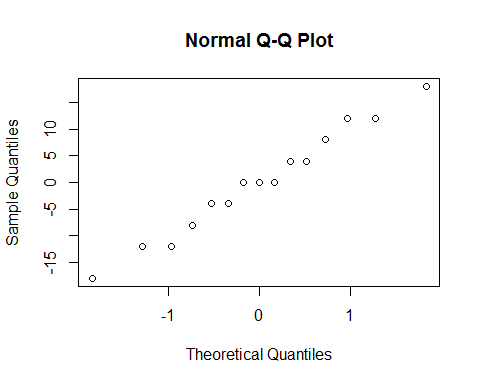
\includegraphics{assignment6_files/figure-latex/unnamed-chunk-12-1.pdf}

Lines have similar slope, which denotes that thorax influences similarly
between activities.

\subsubsection{8.}\label{section-6}

We prefer the analysis with thorax, as it is more complete. Also, it is
possible to detect if there could be a difference in longevity between
groups because of flies with significantly different thorax, instead of
sexual activity. The analysis are fine, both factors do influence
longevity.

\subsubsection{9.}\label{section-7}

\begin{Shaded}
\begin{Highlighting}[]
\KeywordTok{par}\NormalTok{(}\DataTypeTok{mfrow=}\KeywordTok{c}\NormalTok{(}\DecValTok{1}\NormalTok{,}\DecValTok{2}\NormalTok{))}
\KeywordTok{qqnorm}\NormalTok{(}\KeywordTok{residuals}\NormalTok{(flieslm2))}
\KeywordTok{plot}\NormalTok{(}\KeywordTok{fitted}\NormalTok{(flieslm2),}\KeywordTok{residuals}\NormalTok{(flieslm2))}
\end{Highlighting}
\end{Shaded}

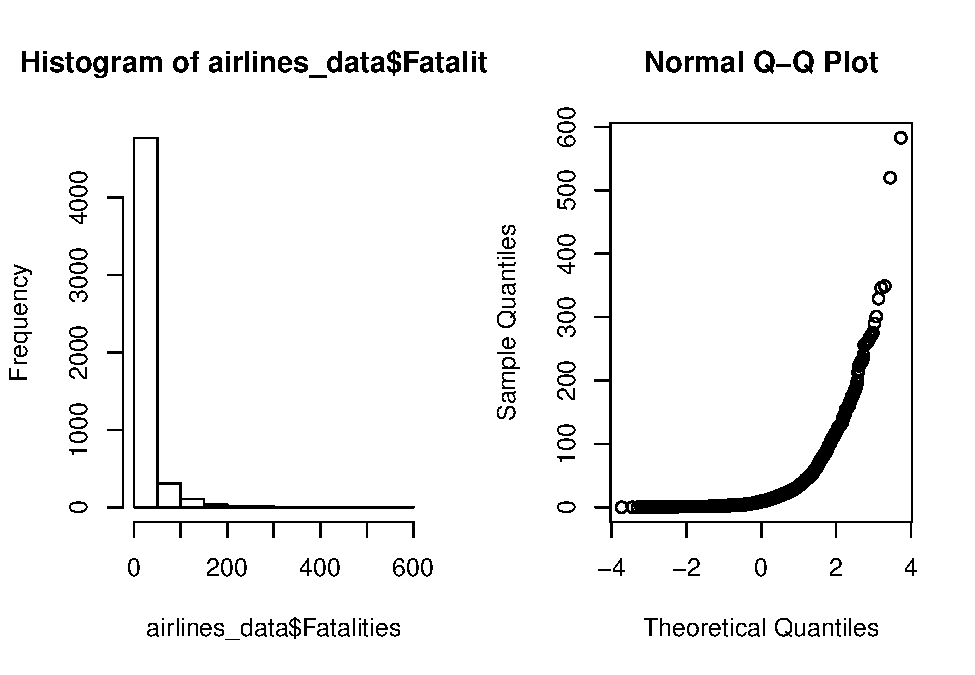
\includegraphics{assignment6_files/figure-latex/unnamed-chunk-13-1.pdf}

Normality is clearly met by the residuals, although heteroscedasticity
is not that clear.

\begin{Shaded}
\begin{Highlighting}[]
\KeywordTok{par}\NormalTok{(}\DataTypeTok{mfrow=}\KeywordTok{c}\NormalTok{(}\DecValTok{1}\NormalTok{,}\DecValTok{2}\NormalTok{))}
\NormalTok{flieslm3 =}\StringTok{ }\KeywordTok{lm}\NormalTok{(longevity~thorax+activity, }\DataTypeTok{data=}\NormalTok{fruitflies)}
\KeywordTok{qqnorm}\NormalTok{(}\KeywordTok{residuals}\NormalTok{(flieslm3))}
\KeywordTok{plot}\NormalTok{(}\KeywordTok{fitted}\NormalTok{(flieslm3),}\KeywordTok{residuals}\NormalTok{(flieslm3))}
\end{Highlighting}
\end{Shaded}

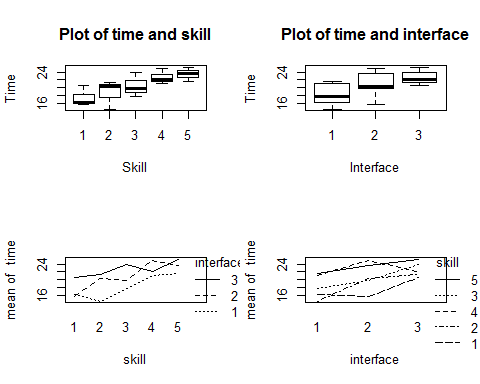
\includegraphics{assignment6_files/figure-latex/unnamed-chunk-14-1.pdf}

In this case heteroscedasticity seems more clear, which may mean that
taking the logarithm of longevity was not a good decition.

\subsection{Exercise 2}\label{exercise-2}

\begin{Shaded}
\begin{Highlighting}[]
\NormalTok{psi=}\KeywordTok{read.table}\NormalTok{(}\StringTok{'psi.txt'}\NormalTok{, }\DataTypeTok{header=}\OtherTok{TRUE}\NormalTok{)}
\end{Highlighting}
\end{Shaded}

\subsubsection{2.}\label{section-8}

\begin{Shaded}
\begin{Highlighting}[]
\NormalTok{psi$psi=}\KeywordTok{factor}\NormalTok{(psi$psi)}
\NormalTok{psi$passed=}\KeywordTok{factor}\NormalTok{(psi$passed)}
\NormalTok{psilm =}\StringTok{ }\KeywordTok{glm}\NormalTok{(passed~psi+gpa, }\DataTypeTok{data=}\NormalTok{psi, }\DataTypeTok{family=}\NormalTok{binomial)}
\end{Highlighting}
\end{Shaded}

\subsubsection{3.}\label{section-9}

\begin{Shaded}
\begin{Highlighting}[]
\KeywordTok{drop1}\NormalTok{(psilm,}\DataTypeTok{test=}\StringTok{"Chisq"}\NormalTok{)}
\end{Highlighting}
\end{Shaded}

\begin{verbatim}
## Single term deletions
## 
## Model:
## passed ~ psi + gpa
##        Df Deviance    AIC    LRT Pr(>Chi)   
## <none>      26.253 32.253                   
## psi     1   32.418 36.418 6.1647 0.013033 * 
## gpa     1   35.342 39.342 9.0885 0.002572 **
## ---
## Signif. codes:  0 '***' 0.001 '**' 0.01 '*' 0.05 '.' 0.1 ' ' 1
\end{verbatim}

\begin{Shaded}
\begin{Highlighting}[]
\KeywordTok{summary}\NormalTok{(psilm)}
\end{Highlighting}
\end{Shaded}

\begin{verbatim}
## 
## Call:
## glm(formula = passed ~ psi + gpa, family = binomial, data = psi)
## 
## Deviance Residuals: 
##     Min       1Q   Median       3Q      Max  
## -1.8396  -0.6282  -0.3045   0.5629   2.0378  
## 
## Coefficients:
##             Estimate Std. Error z value Pr(>|z|)   
## (Intercept)  -11.602      4.213  -2.754  0.00589 **
## psi1           2.338      1.041   2.246  0.02470 * 
## gpa            3.063      1.223   2.505  0.01224 * 
## ---
## Signif. codes:  0 '***' 0.001 '**' 0.01 '*' 0.05 '.' 0.1 ' ' 1
## 
## (Dispersion parameter for binomial family taken to be 1)
## 
##     Null deviance: 41.183  on 31  degrees of freedom
## Residual deviance: 26.253  on 29  degrees of freedom
## AIC: 32.253
## 
## Number of Fisher Scoring iterations: 5
\end{verbatim}

According to the tests above, psi has a significant influence in whether
the student passes or not, and the estimation on when psi is 1 is a
positive number. Therefore, it that influence is positive, which would
mean that psi does improve the learning of students.

\subsubsection{4.}\label{section-10}

\begin{Shaded}
\begin{Highlighting}[]
\CommentTok{# Student with psi with a gpa is 3}
\DecValTok{1}\NormalTok{/(}\DecValTok{1}\NormalTok{+}\KeywordTok{exp}\NormalTok{(-(-}\FloatTok{11.602} \NormalTok{+}\StringTok{ }\FloatTok{2.338}\NormalTok{*}\DecValTok{1} \NormalTok{+}\StringTok{ }\FloatTok{3.063}\NormalTok{*}\DecValTok{3}\NormalTok{)))}
\end{Highlighting}
\end{Shaded}

\begin{verbatim}
## [1] 0.4812588
\end{verbatim}

\begin{Shaded}
\begin{Highlighting}[]
\CommentTok{# Student without psi with a gpa is 3}
\DecValTok{1}\NormalTok{/(}\DecValTok{1}\NormalTok{+}\KeywordTok{exp}\NormalTok{(-(-}\FloatTok{11.602} \NormalTok{+}\StringTok{ }\FloatTok{2.338}\NormalTok{*}\DecValTok{0} \NormalTok{+}\StringTok{ }\FloatTok{3.063}\NormalTok{*}\DecValTok{3}\NormalTok{)))}
\end{Highlighting}
\end{Shaded}

\begin{verbatim}
## [1] 0.08218674
\end{verbatim}

\subsubsection{5.}\label{section-11}

\begin{Shaded}
\begin{Highlighting}[]
\KeywordTok{exp}\NormalTok{(}\FloatTok{2.338}\NormalTok{)}
\end{Highlighting}
\end{Shaded}

\begin{verbatim}
## [1] 10.36049
\end{verbatim}

The odds of passing the assignment rendered by students instructed with
psi is 10.36049. This means that having studied using the psi method
increases the chance of passing the assingment by 10.36049\%. This value
is independent from gpa.

\subsubsection{6.}\label{section-12}

\begin{Shaded}
\begin{Highlighting}[]
\NormalTok{x=}\KeywordTok{matrix}\NormalTok{(}\KeywordTok{c}\NormalTok{(}\DecValTok{3}\NormalTok{,}\DecValTok{15}\NormalTok{,}\DecValTok{8}\NormalTok{,}\DecValTok{6}\NormalTok{),}\DecValTok{2}\NormalTok{,}\DecValTok{2}\NormalTok{)}
\KeywordTok{fisher.test}\NormalTok{(x)}
\end{Highlighting}
\end{Shaded}

\begin{verbatim}
## 
##  Fisher's Exact Test for Count Data
## 
## data:  x
## p-value = 0.0265
## alternative hypothesis: true odds ratio is not equal to 1
## 95 percent confidence interval:
##  0.02016297 0.95505763
## sample estimates:
## odds ratio 
##  0.1605805
\end{verbatim}

15 is the number of students who did not receive psi and didn't showed
improvement. 6 is the number of students who received psi and didn't
show impovement. The hypothesis tested by Fisher's exact test is if
there is independence between the 2 factors (having psi and improving).
This is rejected (p-value \textless{} 0.05) which proves that there is a
dependence between them, and concluding that psi is more helpful to
improve than the previous teaching method.

\subsubsection{7.}\label{section-13}

It does not take into account the amount of improvement found per
student, but besides that it is a correct experiment.

\subsubsection{8.}\label{section-14}

1st: advantage: It takes more information into account, and can estimate
probability of passing having the data of the student. disadvantage: It
is a more complex method and may be sensitive to outliers.

2nd: advantage: It is a simple method to find significance on
improvement. disadvantage: It does not take into account the amount of
improvement found per student

\subsection{Exercise 3}\label{exercise-3}

\subsubsection{1.}\label{section-15}

For this exercise

\begin{Shaded}
\begin{Highlighting}[]
\NormalTok{africa_data=}\KeywordTok{read.table}\NormalTok{(}\StringTok{"africa.txt"}\NormalTok{, }\DataTypeTok{header=}\OtherTok{TRUE}\NormalTok{)}
\KeywordTok{par}\NormalTok{(}\DataTypeTok{mfrow=}\KeywordTok{c}\NormalTok{(}\DecValTok{2}\NormalTok{,}\DecValTok{2}\NormalTok{))}
\KeywordTok{hist}\NormalTok{(}\KeywordTok{rpois}\NormalTok{(}\DecValTok{100}\NormalTok{, }\DataTypeTok{lambda =} \DecValTok{1}\NormalTok{))}
\KeywordTok{hist}\NormalTok{(}\KeywordTok{rpois}\NormalTok{(}\DecValTok{100}\NormalTok{, }\DataTypeTok{lambda =} \DecValTok{5}\NormalTok{))}
\KeywordTok{hist}\NormalTok{(}\KeywordTok{rpois}\NormalTok{(}\DecValTok{100}\NormalTok{, }\DataTypeTok{lambda =} \DecValTok{10}\NormalTok{))}
\KeywordTok{hist}\NormalTok{(}\KeywordTok{rpois}\NormalTok{(}\DecValTok{100}\NormalTok{, }\DataTypeTok{lambda =} \DecValTok{15}\NormalTok{))}
\end{Highlighting}
\end{Shaded}

\includegraphics{assignment6_files/figure-latex/unnamed-chunk-21-1.pdf}

\begin{Shaded}
\begin{Highlighting}[]
\KeywordTok{par}\NormalTok{(}\DataTypeTok{mfrow=}\KeywordTok{c}\NormalTok{(}\DecValTok{2}\NormalTok{,}\DecValTok{2}\NormalTok{))}
\KeywordTok{hist}\NormalTok{(}\KeywordTok{rpois}\NormalTok{(}\DecValTok{1000}\NormalTok{, }\DataTypeTok{lambda =} \DecValTok{1}\NormalTok{))}
\KeywordTok{hist}\NormalTok{(}\KeywordTok{rpois}\NormalTok{(}\DecValTok{1000}\NormalTok{, }\DataTypeTok{lambda =} \DecValTok{5}\NormalTok{))}
\KeywordTok{hist}\NormalTok{(}\KeywordTok{rpois}\NormalTok{(}\DecValTok{1000}\NormalTok{, }\DataTypeTok{lambda =} \DecValTok{10}\NormalTok{))}
\KeywordTok{hist}\NormalTok{(}\KeywordTok{rpois}\NormalTok{(}\DecValTok{1000}\NormalTok{, }\DataTypeTok{lambda =} \DecValTok{15}\NormalTok{))}
\end{Highlighting}
\end{Shaded}

\includegraphics{assignment6_files/figure-latex/unnamed-chunk-22-1.pdf}

\subsubsection{2.}\label{section-16}

\begin{Shaded}
\begin{Highlighting}[]
\KeywordTok{par}\NormalTok{(}\DataTypeTok{mfrow=}\KeywordTok{c}\NormalTok{(}\DecValTok{2}\NormalTok{,}\DecValTok{2}\NormalTok{))}
\KeywordTok{qqnorm}\NormalTok{(}\KeywordTok{rpois}\NormalTok{(}\DecValTok{500}\NormalTok{, }\DataTypeTok{lambda =} \DecValTok{1}\NormalTok{))}
\KeywordTok{qqnorm}\NormalTok{(}\KeywordTok{rpois}\NormalTok{(}\DecValTok{500}\NormalTok{, }\DataTypeTok{lambda =} \DecValTok{15}\NormalTok{))}
\KeywordTok{qqnorm}\NormalTok{(}\KeywordTok{rpois}\NormalTok{(}\DecValTok{100}\NormalTok{, }\DataTypeTok{lambda =} \DecValTok{15}\NormalTok{))}
\KeywordTok{qqnorm}\NormalTok{(}\KeywordTok{rpois}\NormalTok{(}\DecValTok{1000}\NormalTok{, }\DataTypeTok{lambda =} \DecValTok{15}\NormalTok{))}
\end{Highlighting}
\end{Shaded}

\includegraphics{assignment6_files/figure-latex/unnamed-chunk-23-1.pdf}

What can be seen from question one is that as lambda and n increases,
the poisson distribution better approximates a normal distribution. This
is seen in the histograms in question 1 and is further backed up by the
QQ plots. As the poisson distribution gets closer to approximating the
normal distribution, the poisson distributions would be in the same
location-scale family as they would have properties similar to a normal
distribution.

\begin{Shaded}
\begin{Highlighting}[]
\NormalTok{africa_data=}\KeywordTok{read.table}\NormalTok{(}\StringTok{"africa.txt"}\NormalTok{, }\DataTypeTok{header=}\OtherTok{TRUE}\NormalTok{)}
\KeywordTok{par}\NormalTok{(}\DataTypeTok{mfrow=}\KeywordTok{c}\NormalTok{(}\DecValTok{3}\NormalTok{,}\DecValTok{2}\NormalTok{))}
\KeywordTok{hist}\NormalTok{(}\KeywordTok{rpois}\NormalTok{(}\DecValTok{1000}\NormalTok{, }\DataTypeTok{lambda =} \DecValTok{2}\NormalTok{))}
\KeywordTok{hist}\NormalTok{(}\KeywordTok{rpois}\NormalTok{(}\DecValTok{1000}\NormalTok{, }\DataTypeTok{lambda =} \DecValTok{25}\NormalTok{))}
\KeywordTok{hist}\NormalTok{(}\KeywordTok{rpois}\NormalTok{(}\DecValTok{1000}\NormalTok{, }\DataTypeTok{lambda =} \DecValTok{50}\NormalTok{))}
\KeywordTok{hist}\NormalTok{(}\KeywordTok{rpois}\NormalTok{(}\DecValTok{1000}\NormalTok{, }\DataTypeTok{lambda =} \DecValTok{75}\NormalTok{))}
\KeywordTok{hist}\NormalTok{(}\KeywordTok{rpois}\NormalTok{(}\DecValTok{1000}\NormalTok{, }\DataTypeTok{lambda =} \DecValTok{100}\NormalTok{))}
\KeywordTok{hist}\NormalTok{(}\KeywordTok{rpois}\NormalTok{(}\DecValTok{1000}\NormalTok{, }\DataTypeTok{lambda =} \DecValTok{240}\NormalTok{))}
\end{Highlighting}
\end{Shaded}

\includegraphics{assignment6_files/figure-latex/unnamed-chunk-24-1.pdf}

\subsubsection{3}\label{section-17}

\begin{Shaded}
\begin{Highlighting}[]
\CommentTok{#Analysisof variance}
\NormalTok{galaglm_full=}\KeywordTok{glm}\NormalTok{(miltcoup~oligarchy+pollib+parties+pctvote+popn+size+numelec +numregim,}\DataTypeTok{family=}\NormalTok{poisson,}\DataTypeTok{data=}\NormalTok{africa_data)}
\NormalTok{error1 =}\StringTok{ }\KeywordTok{summary}\NormalTok{(galaglm_full)$r.squared}
\KeywordTok{summary}\NormalTok{(galaglm_full)}
\end{Highlighting}
\end{Shaded}

\begin{verbatim}
## 
## Call:
## glm(formula = miltcoup ~ oligarchy + pollib + parties + pctvote + 
##     popn + size + numelec + numregim, family = poisson, data = africa_data)
## 
## Deviance Residuals: 
##     Min       1Q   Median       3Q      Max  
## -1.3443  -0.9542  -0.2587   0.3905   1.6953  
## 
## Coefficients:
##               Estimate Std. Error z value Pr(>|z|)   
## (Intercept) -0.5102693  0.9053301  -0.564  0.57301   
## oligarchy    0.0730814  0.0345958   2.112  0.03465 * 
## pollib      -0.7129779  0.2725635  -2.616  0.00890 **
## parties      0.0307739  0.0111873   2.751  0.00595 **
## pctvote      0.0138722  0.0097526   1.422  0.15491   
## popn         0.0093429  0.0065950   1.417  0.15658   
## size        -0.0001900  0.0002485  -0.765  0.44447   
## numelec     -0.0160783  0.0654842  -0.246  0.80605   
## numregim     0.1917349  0.2292890   0.836  0.40303   
## ---
## Signif. codes:  0 '***' 0.001 '**' 0.01 '*' 0.05 '.' 0.1 ' ' 1
## 
## (Dispersion parameter for poisson family taken to be 1)
## 
##     Null deviance: 65.945  on 35  degrees of freedom
## Residual deviance: 28.668  on 27  degrees of freedom
## AIC: 111.48
## 
## Number of Fisher Scoring iterations: 6
\end{verbatim}

\subsubsection{4.}\label{section-18}

Removing numelec has it had the gighest p-value.

\begin{Shaded}
\begin{Highlighting}[]
\CommentTok{#Analysisof variance}
\NormalTok{galaglm=}\KeywordTok{glm}\NormalTok{(miltcoup~oligarchy+pollib+parties+pctvote+popn+size +numregim,}\DataTypeTok{family=}\NormalTok{poisson,}\DataTypeTok{data=}\NormalTok{africa_data)}
\KeywordTok{summary}\NormalTok{(galaglm)}
\end{Highlighting}
\end{Shaded}

\begin{verbatim}
## 
## Call:
## glm(formula = miltcoup ~ oligarchy + pollib + parties + pctvote + 
##     popn + size + numregim, family = poisson, data = africa_data)
## 
## Deviance Residuals: 
##     Min       1Q   Median       3Q      Max  
## -1.3997  -0.9381  -0.2666   0.4220   1.6998  
## 
## Coefficients:
##               Estimate Std. Error z value Pr(>|z|)   
## (Intercept) -0.6078028  0.8239267  -0.738  0.46070   
## oligarchy    0.0781368  0.0277656   2.814  0.00489 **
## pollib      -0.6773897  0.2290130  -2.958  0.00310 **
## parties      0.0296786  0.0102888   2.885  0.00392 **
## pctvote      0.0131290  0.0092895   1.413  0.15756   
## popn         0.0089313  0.0063746   1.401  0.16120   
## size        -0.0002021  0.0002436  -0.830  0.40682   
## numregim     0.1758198  0.2210498   0.795  0.42639   
## ---
## Signif. codes:  0 '***' 0.001 '**' 0.01 '*' 0.05 '.' 0.1 ' ' 1
## 
## (Dispersion parameter for poisson family taken to be 1)
## 
##     Null deviance: 65.945  on 35  degrees of freedom
## Residual deviance: 28.728  on 28  degrees of freedom
## AIC: 109.54
## 
## Number of Fisher Scoring iterations: 5
\end{verbatim}

Removing numregim.

\begin{Shaded}
\begin{Highlighting}[]
\NormalTok{galaglm=}\KeywordTok{glm}\NormalTok{(miltcoup~oligarchy+pollib+parties+pctvote+popn+size,}\DataTypeTok{family=}\NormalTok{poisson,}\DataTypeTok{data=}\NormalTok{africa_data)}
\KeywordTok{summary}\NormalTok{(galaglm)}
\end{Highlighting}
\end{Shaded}

\begin{verbatim}
## 
## Call:
## glm(formula = miltcoup ~ oligarchy + pollib + parties + pctvote + 
##     popn + size, family = poisson, data = africa_data)
## 
## Deviance Residuals: 
##     Min       1Q   Median       3Q      Max  
## -1.3522  -0.9651  -0.1945   0.4833   1.6179  
## 
## Coefficients:
##               Estimate Std. Error z value Pr(>|z|)    
## (Intercept) -0.1126871  0.5163030  -0.218 0.827228    
## oligarchy    0.0859620  0.0259100   3.318 0.000908 ***
## pollib      -0.6894029  0.2278572  -3.026 0.002481 ** 
## parties      0.0291944  0.0101954   2.863 0.004190 ** 
## pctvote      0.0141588  0.0091980   1.539 0.123723    
## popn         0.0062736  0.0053994   1.162 0.245272    
## size        -0.0001950  0.0002425  -0.804 0.421378    
## ---
## Signif. codes:  0 '***' 0.001 '**' 0.01 '*' 0.05 '.' 0.1 ' ' 1
## 
## (Dispersion parameter for poisson family taken to be 1)
## 
##     Null deviance: 65.945  on 35  degrees of freedom
## Residual deviance: 29.363  on 29  degrees of freedom
## AIC: 108.17
## 
## Number of Fisher Scoring iterations: 5
\end{verbatim}

Removing size.

\begin{Shaded}
\begin{Highlighting}[]
\NormalTok{galaglm=}\KeywordTok{glm}\NormalTok{(miltcoup~oligarchy+pollib+parties+pctvote+popn,}\DataTypeTok{family=}\NormalTok{poisson,}\DataTypeTok{data=}\NormalTok{africa_data)}
\KeywordTok{summary}\NormalTok{(galaglm)}
\end{Highlighting}
\end{Shaded}

\begin{verbatim}
## 
## Call:
## glm(formula = miltcoup ~ oligarchy + pollib + parties + pctvote + 
##     popn, family = poisson, data = africa_data)
## 
## Deviance Residuals: 
##     Min       1Q   Median       3Q      Max  
## -1.4109  -0.9943  -0.1399   0.5516   1.6125  
## 
## Coefficients:
##              Estimate Std. Error z value Pr(>|z|)   
## (Intercept) -0.244466   0.495708  -0.493  0.62190   
## oligarchy    0.083168   0.025437   3.270  0.00108 **
## pollib      -0.652830   0.221234  -2.951  0.00317 **
## parties      0.029800   0.010294   2.895  0.00379 **
## pctvote      0.013842   0.009282   1.491  0.13591   
## popn         0.005587   0.005378   1.039  0.29883   
## ---
## Signif. codes:  0 '***' 0.001 '**' 0.01 '*' 0.05 '.' 0.1 ' ' 1
## 
## (Dispersion parameter for poisson family taken to be 1)
## 
##     Null deviance: 65.945  on 35  degrees of freedom
## Residual deviance: 30.044  on 30  degrees of freedom
## AIC: 106.85
## 
## Number of Fisher Scoring iterations: 5
\end{verbatim}

Removing popn.

\begin{Shaded}
\begin{Highlighting}[]
\NormalTok{galaglm=}\KeywordTok{glm}\NormalTok{(miltcoup~oligarchy+pollib+parties+pctvote,}\DataTypeTok{family=}\NormalTok{poisson,}\DataTypeTok{data=}\NormalTok{africa_data)}
\KeywordTok{summary}\NormalTok{(galaglm)}
\end{Highlighting}
\end{Shaded}

\begin{verbatim}
## 
## Call:
## glm(formula = miltcoup ~ oligarchy + pollib + parties + pctvote, 
##     family = poisson, data = africa_data)
## 
## Deviance Residuals: 
##     Min       1Q   Median       3Q      Max  
## -1.5456  -0.9841  -0.1881   0.5948   1.6705  
## 
## Coefficients:
##              Estimate Std. Error z value Pr(>|z|)    
## (Intercept) -0.093657   0.463279  -0.202  0.83979    
## oligarchy    0.095358   0.022421   4.253 2.11e-05 ***
## pollib      -0.666615   0.217564  -3.064  0.00218 ** 
## parties      0.025630   0.009502   2.697  0.00699 ** 
## pctvote      0.012134   0.009056   1.340  0.18031    
## ---
## Signif. codes:  0 '***' 0.001 '**' 0.01 '*' 0.05 '.' 0.1 ' ' 1
## 
## (Dispersion parameter for poisson family taken to be 1)
## 
##     Null deviance: 65.945  on 35  degrees of freedom
## Residual deviance: 31.081  on 31  degrees of freedom
## AIC: 105.89
## 
## Number of Fisher Scoring iterations: 5
\end{verbatim}

And finally removing pctvote.

\begin{Shaded}
\begin{Highlighting}[]
\NormalTok{galaglm=}\KeywordTok{glm}\NormalTok{(miltcoup~oligarchy+pollib+parties,}\DataTypeTok{family=}\NormalTok{poisson,}\DataTypeTok{data=}\NormalTok{africa_data)}
\KeywordTok{summary}\NormalTok{(galaglm)}
\end{Highlighting}
\end{Shaded}

\begin{verbatim}
## 
## Call:
## glm(formula = miltcoup ~ oligarchy + pollib + parties, family = poisson, 
##     data = africa_data)
## 
## Deviance Residuals: 
##     Min       1Q   Median       3Q      Max  
## -1.3583  -1.0424  -0.2863   0.6278   1.7517  
## 
## Coefficients:
##              Estimate Std. Error z value Pr(>|z|)    
## (Intercept)  0.251377   0.372689   0.674  0.50000    
## oligarchy    0.092622   0.021779   4.253 2.11e-05 ***
## pollib      -0.574103   0.204383  -2.809  0.00497 ** 
## parties      0.022059   0.008955   2.463  0.01377 *  
## ---
## Signif. codes:  0 '***' 0.001 '**' 0.01 '*' 0.05 '.' 0.1 ' ' 1
## 
## (Dispersion parameter for poisson family taken to be 1)
## 
##     Null deviance: 65.945  on 35  degrees of freedom
## Residual deviance: 32.856  on 32  degrees of freedom
## AIC: 105.66
## 
## Number of Fisher Scoring iterations: 5
\end{verbatim}

\subsubsection{5.}\label{section-19}

\begin{Shaded}
\begin{Highlighting}[]
\KeywordTok{par}\NormalTok{(}\DataTypeTok{mfrow=}\KeywordTok{c}\NormalTok{(}\DecValTok{2}\NormalTok{,}\DecValTok{2}\NormalTok{))}
\KeywordTok{attach}\NormalTok{(africa_data)}
\KeywordTok{plot}\NormalTok{(}\KeywordTok{fitted}\NormalTok{(galaglm),}\KeywordTok{residuals}\NormalTok{(galaglm))}
\KeywordTok{plot}\NormalTok{(}\KeywordTok{residuals}\NormalTok{(galaglm),parties)}
\KeywordTok{plot}\NormalTok{(}\KeywordTok{residuals}\NormalTok{(galaglm),pollib)}
\KeywordTok{plot}\NormalTok{(}\KeywordTok{residuals}\NormalTok{(galaglm),oligarchy)}
\end{Highlighting}
\end{Shaded}

\includegraphics{assignment6_files/figure-latex/unnamed-chunk-31-1.pdf}

\begin{Shaded}
\begin{Highlighting}[]
\KeywordTok{par}\NormalTok{(}\DataTypeTok{mfrow=}\KeywordTok{c}\NormalTok{(}\DecValTok{1}\NormalTok{,}\DecValTok{3}\NormalTok{))}
\KeywordTok{plot}\NormalTok{(}\KeywordTok{residuals}\NormalTok{(galaglm_full),parties)}
\KeywordTok{plot}\NormalTok{(}\KeywordTok{log}\NormalTok{(}\KeywordTok{fitted}\NormalTok{(galaglm)),}\KeywordTok{residuals}\NormalTok{(galaglm))}
\KeywordTok{plot}\NormalTok{(}\KeywordTok{log}\NormalTok{(}\KeywordTok{fitted}\NormalTok{(galaglm)),}\KeywordTok{residuals}\NormalTok{(galaglm,}\DataTypeTok{type=}\StringTok{"response"}\NormalTok{))}
\end{Highlighting}
\end{Shaded}

\includegraphics{assignment6_files/figure-latex/unnamed-chunk-32-1.pdf}

The response residuals clearly increase with the (logarithm) of the
fitted values, as expected under a Poisson model.

Next, the model from Q3 will be investigated to see if it follows the
same pattern.

\begin{Shaded}
\begin{Highlighting}[]
\KeywordTok{par}\NormalTok{(}\DataTypeTok{mfrow=}\KeywordTok{c}\NormalTok{(}\DecValTok{1}\NormalTok{,}\DecValTok{3}\NormalTok{))}
\KeywordTok{plot}\NormalTok{(}\KeywordTok{residuals}\NormalTok{(galaglm_full),parties)}
\KeywordTok{plot}\NormalTok{(}\KeywordTok{log}\NormalTok{(}\KeywordTok{fitted}\NormalTok{(galaglm_full)),}\KeywordTok{residuals}\NormalTok{(galaglm_full))}
\KeywordTok{plot}\NormalTok{(}\KeywordTok{log}\NormalTok{(}\KeywordTok{fitted}\NormalTok{(galaglm_full)),}\KeywordTok{residuals}\NormalTok{(galaglm_full,}\DataTypeTok{type=}\StringTok{"response"}\NormalTok{))}
\end{Highlighting}
\end{Shaded}

\includegraphics{assignment6_files/figure-latex/unnamed-chunk-33-1.pdf}

While the response residuals clearly increase with the logarithm of the
fitted values, the step down approach looks to contain less clear
patterns in it's data. In the full model with all explanatory variables,
there looks to be much clearer linear structures within the data
compared to the step down model. This could be due to the removed
variables. During the process of the step down approach in Q4 what can
be seen is that some of the variables become less significant as
variables are removed. For example, in the last step the variable
pctvote is removed. This reduces the p-value of the variable parties. By
removing pctvote, the relationship between pctvote and parties is
removed which could affect the model if the is a dependency between
these two variables.

\begin{Shaded}
\begin{Highlighting}[]
\KeywordTok{pairs}\NormalTok{(pctvote~parties)}
\end{Highlighting}
\end{Shaded}

\includegraphics{assignment6_files/figure-latex/unnamed-chunk-34-1.pdf}

However, from the pairs graph there does not seem to be a correlation.


\end{document}
